% Options for packages loaded elsewhere
\PassOptionsToPackage{unicode}{hyperref}
\PassOptionsToPackage{hyphens}{url}
\PassOptionsToPackage{dvipsnames,svgnames,x11names}{xcolor}
%
\documentclass[
  letterpaper,
  DIV=11,
  numbers=noendperiod]{scrartcl}

\usepackage{amsmath,amssymb}
\usepackage{iftex}
\ifPDFTeX
  \usepackage[T1]{fontenc}
  \usepackage[utf8]{inputenc}
  \usepackage{textcomp} % provide euro and other symbols
\else % if luatex or xetex
  \usepackage{unicode-math}
  \defaultfontfeatures{Scale=MatchLowercase}
  \defaultfontfeatures[\rmfamily]{Ligatures=TeX,Scale=1}
\fi
\usepackage{lmodern}
\ifPDFTeX\else  
    % xetex/luatex font selection
\fi
% Use upquote if available, for straight quotes in verbatim environments
\IfFileExists{upquote.sty}{\usepackage{upquote}}{}
\IfFileExists{microtype.sty}{% use microtype if available
  \usepackage[]{microtype}
  \UseMicrotypeSet[protrusion]{basicmath} % disable protrusion for tt fonts
}{}
\makeatletter
\@ifundefined{KOMAClassName}{% if non-KOMA class
  \IfFileExists{parskip.sty}{%
    \usepackage{parskip}
  }{% else
    \setlength{\parindent}{0pt}
    \setlength{\parskip}{6pt plus 2pt minus 1pt}}
}{% if KOMA class
  \KOMAoptions{parskip=half}}
\makeatother
\usepackage{xcolor}
\setlength{\emergencystretch}{3em} % prevent overfull lines
\setcounter{secnumdepth}{-\maxdimen} % remove section numbering
% Make \paragraph and \subparagraph free-standing
\ifx\paragraph\undefined\else
  \let\oldparagraph\paragraph
  \renewcommand{\paragraph}[1]{\oldparagraph{#1}\mbox{}}
\fi
\ifx\subparagraph\undefined\else
  \let\oldsubparagraph\subparagraph
  \renewcommand{\subparagraph}[1]{\oldsubparagraph{#1}\mbox{}}
\fi

\usepackage{color}
\usepackage{fancyvrb}
\newcommand{\VerbBar}{|}
\newcommand{\VERB}{\Verb[commandchars=\\\{\}]}
\DefineVerbatimEnvironment{Highlighting}{Verbatim}{commandchars=\\\{\}}
% Add ',fontsize=\small' for more characters per line
\usepackage{framed}
\definecolor{shadecolor}{RGB}{241,243,245}
\newenvironment{Shaded}{\begin{snugshade}}{\end{snugshade}}
\newcommand{\AlertTok}[1]{\textcolor[rgb]{0.68,0.00,0.00}{#1}}
\newcommand{\AnnotationTok}[1]{\textcolor[rgb]{0.37,0.37,0.37}{#1}}
\newcommand{\AttributeTok}[1]{\textcolor[rgb]{0.40,0.45,0.13}{#1}}
\newcommand{\BaseNTok}[1]{\textcolor[rgb]{0.68,0.00,0.00}{#1}}
\newcommand{\BuiltInTok}[1]{\textcolor[rgb]{0.00,0.23,0.31}{#1}}
\newcommand{\CharTok}[1]{\textcolor[rgb]{0.13,0.47,0.30}{#1}}
\newcommand{\CommentTok}[1]{\textcolor[rgb]{0.37,0.37,0.37}{#1}}
\newcommand{\CommentVarTok}[1]{\textcolor[rgb]{0.37,0.37,0.37}{\textit{#1}}}
\newcommand{\ConstantTok}[1]{\textcolor[rgb]{0.56,0.35,0.01}{#1}}
\newcommand{\ControlFlowTok}[1]{\textcolor[rgb]{0.00,0.23,0.31}{#1}}
\newcommand{\DataTypeTok}[1]{\textcolor[rgb]{0.68,0.00,0.00}{#1}}
\newcommand{\DecValTok}[1]{\textcolor[rgb]{0.68,0.00,0.00}{#1}}
\newcommand{\DocumentationTok}[1]{\textcolor[rgb]{0.37,0.37,0.37}{\textit{#1}}}
\newcommand{\ErrorTok}[1]{\textcolor[rgb]{0.68,0.00,0.00}{#1}}
\newcommand{\ExtensionTok}[1]{\textcolor[rgb]{0.00,0.23,0.31}{#1}}
\newcommand{\FloatTok}[1]{\textcolor[rgb]{0.68,0.00,0.00}{#1}}
\newcommand{\FunctionTok}[1]{\textcolor[rgb]{0.28,0.35,0.67}{#1}}
\newcommand{\ImportTok}[1]{\textcolor[rgb]{0.00,0.46,0.62}{#1}}
\newcommand{\InformationTok}[1]{\textcolor[rgb]{0.37,0.37,0.37}{#1}}
\newcommand{\KeywordTok}[1]{\textcolor[rgb]{0.00,0.23,0.31}{#1}}
\newcommand{\NormalTok}[1]{\textcolor[rgb]{0.00,0.23,0.31}{#1}}
\newcommand{\OperatorTok}[1]{\textcolor[rgb]{0.37,0.37,0.37}{#1}}
\newcommand{\OtherTok}[1]{\textcolor[rgb]{0.00,0.23,0.31}{#1}}
\newcommand{\PreprocessorTok}[1]{\textcolor[rgb]{0.68,0.00,0.00}{#1}}
\newcommand{\RegionMarkerTok}[1]{\textcolor[rgb]{0.00,0.23,0.31}{#1}}
\newcommand{\SpecialCharTok}[1]{\textcolor[rgb]{0.37,0.37,0.37}{#1}}
\newcommand{\SpecialStringTok}[1]{\textcolor[rgb]{0.13,0.47,0.30}{#1}}
\newcommand{\StringTok}[1]{\textcolor[rgb]{0.13,0.47,0.30}{#1}}
\newcommand{\VariableTok}[1]{\textcolor[rgb]{0.07,0.07,0.07}{#1}}
\newcommand{\VerbatimStringTok}[1]{\textcolor[rgb]{0.13,0.47,0.30}{#1}}
\newcommand{\WarningTok}[1]{\textcolor[rgb]{0.37,0.37,0.37}{\textit{#1}}}

\providecommand{\tightlist}{%
  \setlength{\itemsep}{0pt}\setlength{\parskip}{0pt}}\usepackage{longtable,booktabs,array}
\usepackage{calc} % for calculating minipage widths
% Correct order of tables after \paragraph or \subparagraph
\usepackage{etoolbox}
\makeatletter
\patchcmd\longtable{\par}{\if@noskipsec\mbox{}\fi\par}{}{}
\makeatother
% Allow footnotes in longtable head/foot
\IfFileExists{footnotehyper.sty}{\usepackage{footnotehyper}}{\usepackage{footnote}}
\makesavenoteenv{longtable}
\usepackage{graphicx}
\makeatletter
\def\maxwidth{\ifdim\Gin@nat@width>\linewidth\linewidth\else\Gin@nat@width\fi}
\def\maxheight{\ifdim\Gin@nat@height>\textheight\textheight\else\Gin@nat@height\fi}
\makeatother
% Scale images if necessary, so that they will not overflow the page
% margins by default, and it is still possible to overwrite the defaults
% using explicit options in \includegraphics[width, height, ...]{}
\setkeys{Gin}{width=\maxwidth,height=\maxheight,keepaspectratio}
% Set default figure placement to htbp
\makeatletter
\def\fps@figure{htbp}
\makeatother

\usepackage{booktabs}
\usepackage{longtable}
\usepackage{array}
\usepackage{multirow}
\usepackage{wrapfig}
\usepackage{float}
\usepackage{colortbl}
\usepackage{pdflscape}
\usepackage{tabu}
\usepackage{threeparttable}
\usepackage{threeparttablex}
\usepackage[normalem]{ulem}
\usepackage{makecell}
\usepackage{xcolor}
\usepackage{wrapfig}
\usepackage{colortbl}
 \makeatletter
 \renewenvironment{table}%
   {\renewcommand\familydefault\sfdefault
    \@float{table}}
   {\end@float}
 \renewenvironment{figure}%
   {\renewcommand\familydefault\sfdefault
    \@float{figure}}
   {\end@float}
 \makeatother
\KOMAoption{captions}{tableheading}
\makeatletter
\makeatother
\makeatletter
\makeatother
\makeatletter
\@ifpackageloaded{caption}{}{\usepackage{caption}}
\AtBeginDocument{%
\ifdefined\contentsname
  \renewcommand*\contentsname{Table of contents}
\else
  \newcommand\contentsname{Table of contents}
\fi
\ifdefined\listfigurename
  \renewcommand*\listfigurename{List of Figures}
\else
  \newcommand\listfigurename{List of Figures}
\fi
\ifdefined\listtablename
  \renewcommand*\listtablename{List of Tables}
\else
  \newcommand\listtablename{List of Tables}
\fi
\ifdefined\figurename
  \renewcommand*\figurename{Figure}
\else
  \newcommand\figurename{Figure}
\fi
\ifdefined\tablename
  \renewcommand*\tablename{Table}
\else
  \newcommand\tablename{Table}
\fi
}
\@ifpackageloaded{float}{}{\usepackage{float}}
\floatstyle{ruled}
\@ifundefined{c@chapter}{\newfloat{codelisting}{h}{lop}}{\newfloat{codelisting}{h}{lop}[chapter]}
\floatname{codelisting}{Listing}
\newcommand*\listoflistings{\listof{codelisting}{List of Listings}}
\makeatother
\makeatletter
\@ifpackageloaded{caption}{}{\usepackage{caption}}
\@ifpackageloaded{subcaption}{}{\usepackage{subcaption}}
\makeatother
\makeatletter
\@ifpackageloaded{tcolorbox}{}{\usepackage[skins,breakable]{tcolorbox}}
\makeatother
\makeatletter
\@ifundefined{shadecolor}{\definecolor{shadecolor}{rgb}{.97, .97, .97}}
\makeatother
\makeatletter
\makeatother
\makeatletter
\makeatother
\ifLuaTeX
  \usepackage{selnolig}  % disable illegal ligatures
\fi
\IfFileExists{bookmark.sty}{\usepackage{bookmark}}{\usepackage{hyperref}}
\IfFileExists{xurl.sty}{\usepackage{xurl}}{} % add URL line breaks if available
\urlstyle{same} % disable monospaced font for URLs
\hypersetup{
  pdftitle={Tests},
  colorlinks=true,
  linkcolor={blue},
  filecolor={Maroon},
  citecolor={Blue},
  urlcolor={Blue},
  pdfcreator={LaTeX via pandoc}}

\title{Tests}
\author{}
\date{}

\begin{document}
\maketitle
\ifdefined\Shaded\renewenvironment{Shaded}{\begin{tcolorbox}[frame hidden, interior hidden, enhanced, borderline west={3pt}{0pt}{shadecolor}, breakable, boxrule=0pt, sharp corners]}{\end{tcolorbox}}\fi

\begin{Shaded}
\begin{Highlighting}[]
\CommentTok{\# read in master data}
\NormalTok{bhet\_master\_data }\OtherTok{\textless{}{-}} \FunctionTok{osf\_retrieve\_node}\NormalTok{(}\StringTok{"vxur5"}\NormalTok{)}
\NormalTok{bhet\_master\_data }\SpecialCharTok{\%\textgreater{}\%}
  \FunctionTok{osf\_ls\_files}\NormalTok{(}\StringTok{"Master Dataset (Seasons 1{-}4)"}\NormalTok{,}
               \AttributeTok{pattern =} \StringTok{"csv"}\NormalTok{) }\SpecialCharTok{\%\textgreater{}\%}
  \FunctionTok{osf\_download}\NormalTok{(}\AttributeTok{path =} \FunctionTok{here}\NormalTok{(}\StringTok{"data{-}clean"}\NormalTok{),}
               \AttributeTok{conflicts =} \StringTok{"overwrite"}\NormalTok{)}

\CommentTok{\# read in data for Aim 1}
\NormalTok{aim\_1 }\OtherTok{\textless{}{-}} \FunctionTok{osf\_retrieve\_node}\NormalTok{(}\StringTok{"qsmbr"}\NormalTok{)}
\NormalTok{aim\_1 }\SpecialCharTok{\%\textgreater{}\%}
  \FunctionTok{osf\_ls\_files}\NormalTok{(}\StringTok{"Air pollution"}\NormalTok{,}
    \AttributeTok{pattern =} \StringTok{"csv"}\NormalTok{) }\SpecialCharTok{\%\textgreater{}\%}
  \FunctionTok{osf\_download}\NormalTok{(}\AttributeTok{path =} \FunctionTok{here}\NormalTok{(}\StringTok{"data{-}clean"}\NormalTok{),}
               \AttributeTok{conflicts =} \StringTok{"overwrite"}\NormalTok{)}
\end{Highlighting}
\end{Shaded}

Read in data

Make a table

\begin{table}

\end{table}

See \textbf{?@tbl-table1} for details.

Now try for the kable version:

\begin{table}

\end{table}

\begin{table}

\end{table}

Another DiD table

See \textbf{?@tbl-table3} for more.

\begin{table}

\end{table}

\newpage

The source profiles for the four-factor solution are presented in Figure
X. The first source was identified as dust by high percentages of
crustal elements like wi-Ca, Si, and wi-Mg. The second source was
constituted of non-sulfate sulfur as well as secondary inorganic ions
(ammonium, nitrate, and sulfate). Non-sulfate sulfur is a tracer for
primary coal combustion, while secondary inorganic ions indicate a
secondary source. Since coal combustion is a major source of energy in
our study area, it is likely that the second source is a mixture of
primary and secondary emissions that originate from coal and other
sulfurous fuel combustion.

\begin{wrapfigure}{R}{0.7\textwidth}
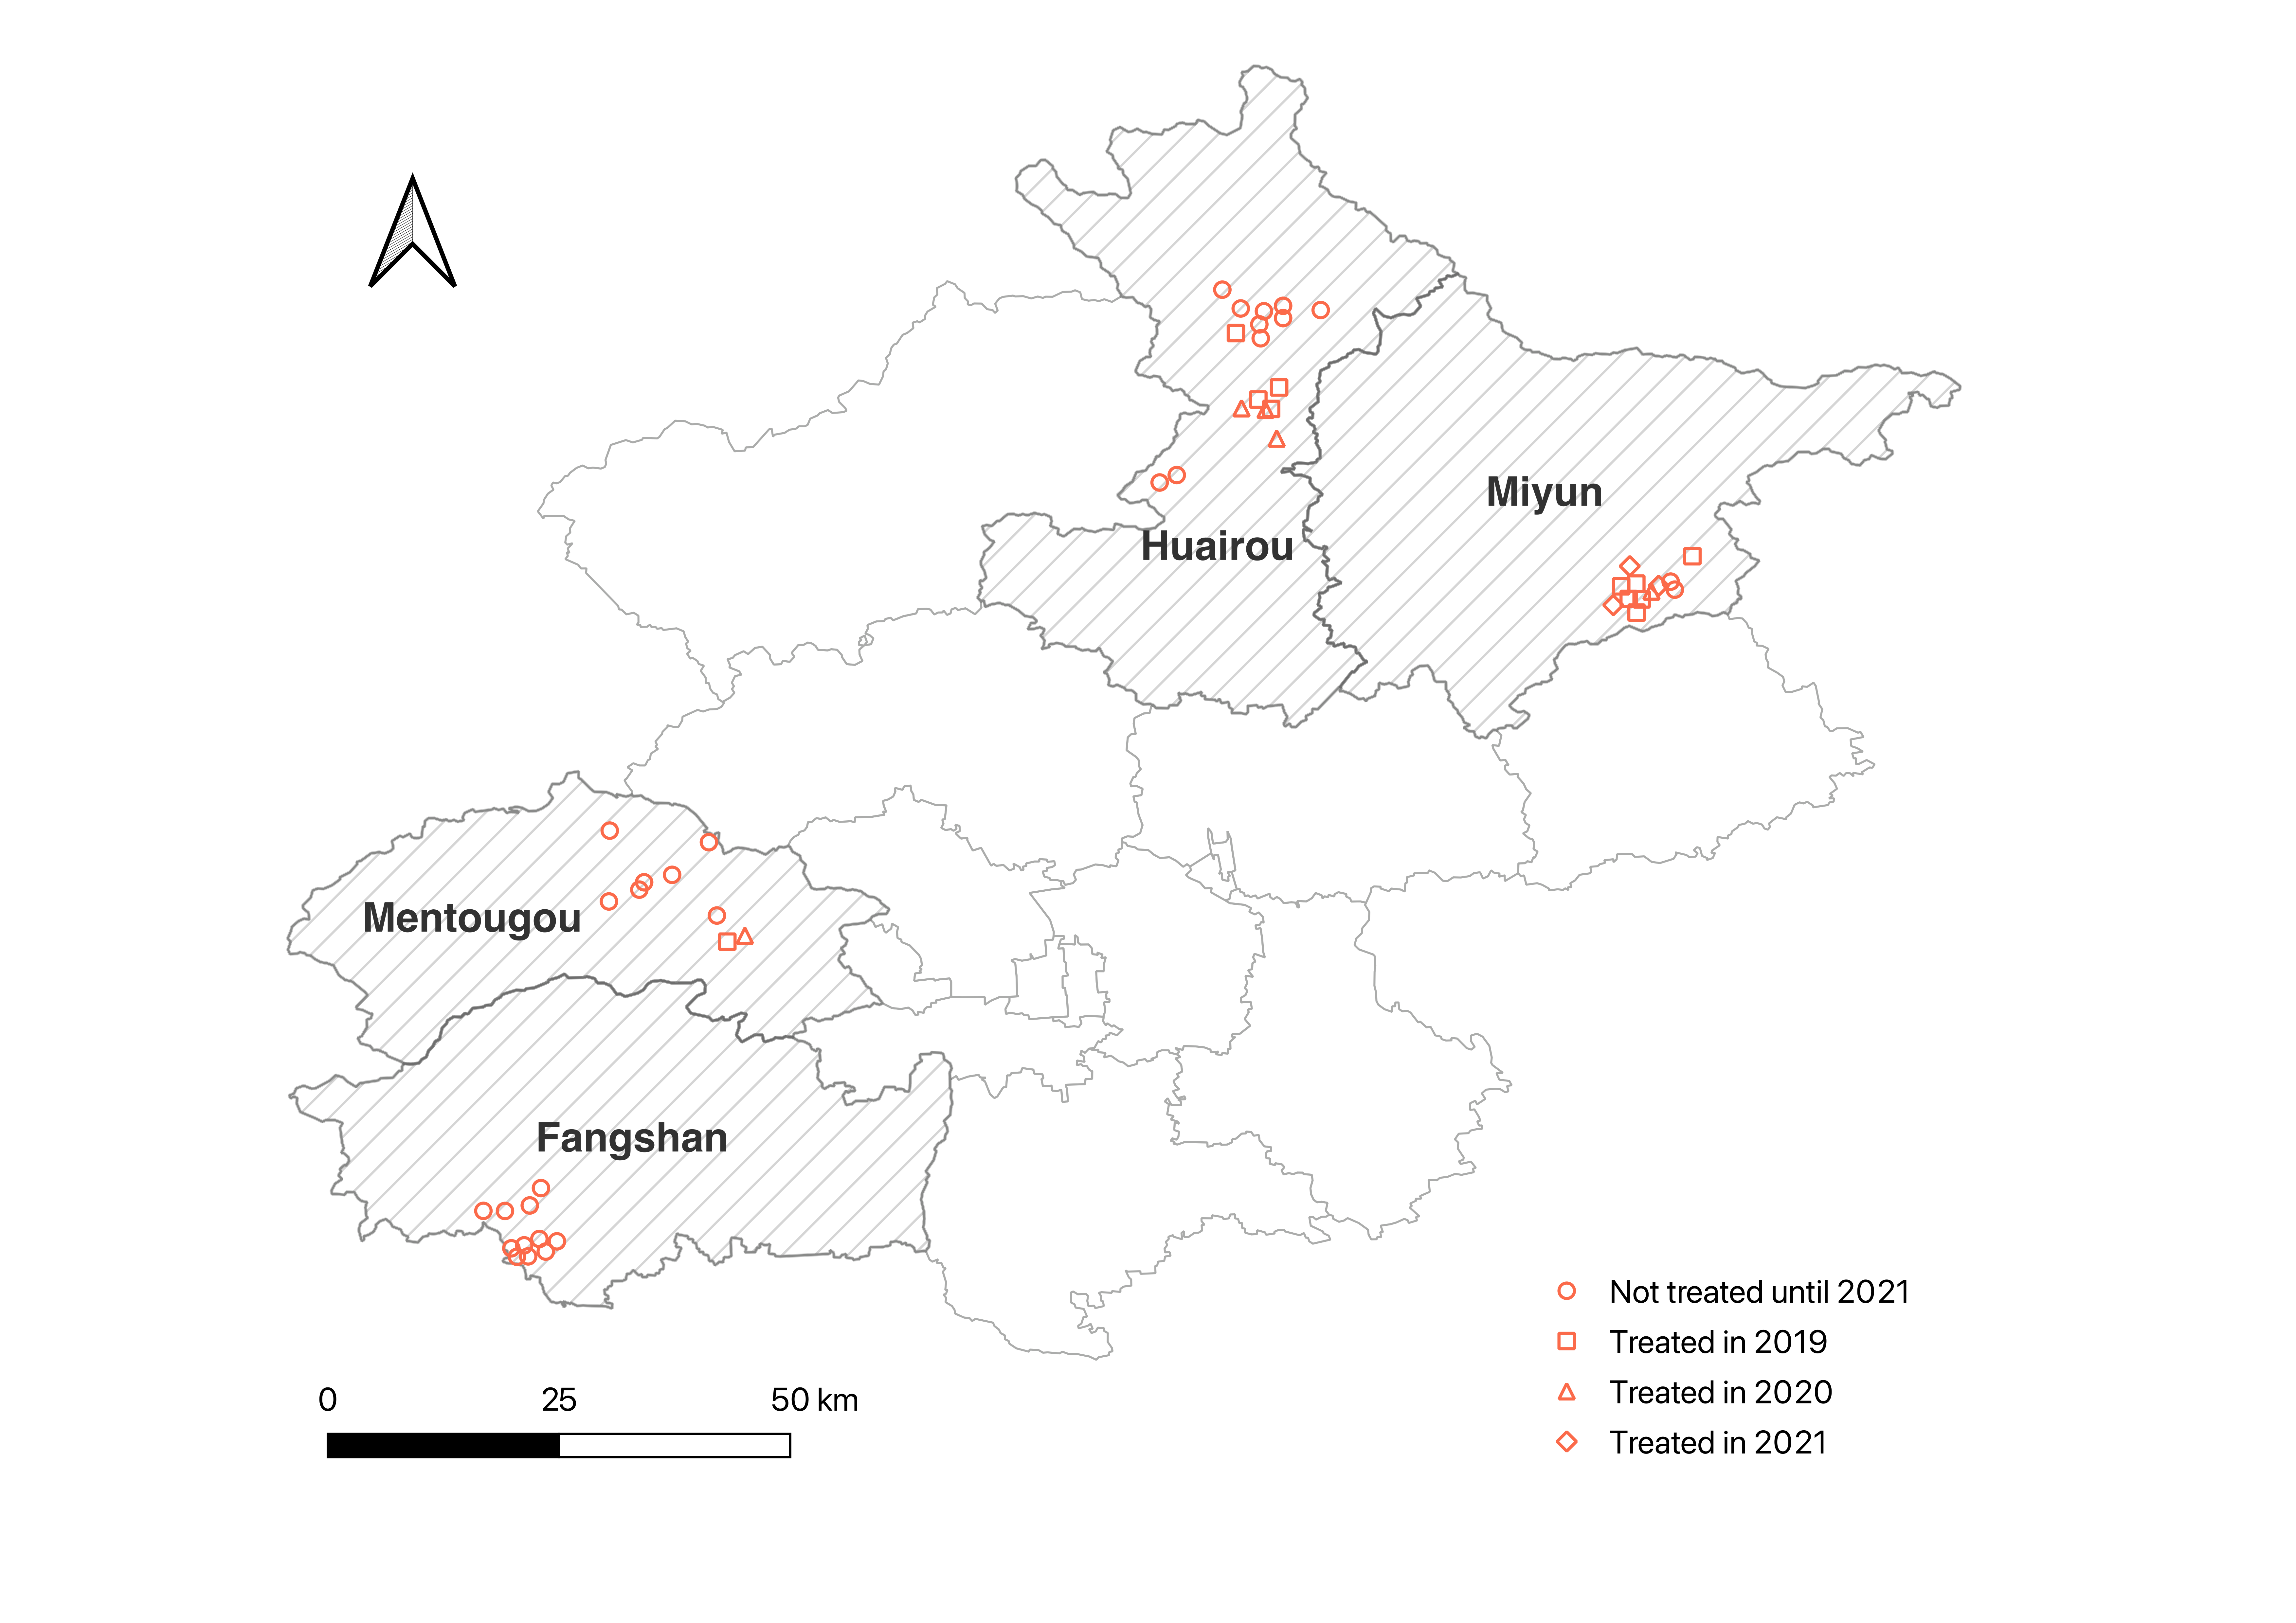
\includegraphics[width=0.7\textwidth]{images/policy-implementation-map.png}
\caption{\label{fig-map}{Google scholar metrics}}
\end{wrapfigure}

Additionally, in Figure\ref{fig-map} for details. the mean source
contribution of the second source is higher in outdoor than personal
exposure measurements. Secondary formation occurs outdoors in the
presence of sunlight, so higher outdoor concentrations compared to
personal exposure further support our naming the second source and
sulfur secondary. The third source had high percentages of ws-Ca nd Al,
which in our study region, has been found to be indicative of
transported dust from dust storms that can occur in the spring. While
our samples were collected during winter months only, it is possible
that transported dust from previous years still remained. The fourth
source was characterized by high percentages of tracers for both coal
(OC, wi-K, chloride, Pb) and biomass combustion (EC, ws-K). Coal and
biomass combustion is common in our study setting so this source is
likely a mixture of the two combustion sources.

Another example

\hypertarget{tbl-fuel}{}
\begin{table}
\caption{\label{tbl-fuel}Policy impacts on self-reported fuel use (kg) }\tabularnewline

\centering
\begin{tabular}{>{\centering\arraybackslash}p{1.5cm}>{\centering\arraybackslash}p{1.5cm}cccc}
\toprule
\multicolumn{2}{c}{ } & \multicolumn{2}{c}{Coal\textsuperscript{a}} & \multicolumn{2}{c}{Biomass\textsuperscript{b}} \\
\cmidrule(l{3pt}r{3pt}){3-4} \cmidrule(l{3pt}r{3pt}){5-6}
Cohort & Time & ATT & (95\%CI) & ATT & (95\%CI)\\
\midrule
\addlinespace[0.3em]
\multicolumn{6}{l}{\textbf{Average ATT}}\\
All & All & -2361 & (-2677, -2044) & -487 & (-805, -168)\\
\addlinespace[0.3em]
\multicolumn{6}{l}{\textbf{Cohort-Time ATTs}}\\
2019 & 2019 & -2631 & (-2913, -2348) & -653 & (-991, -315)\\
2019 & 2021 & -2416 & (-2847, -1984) & -633 & (-1201, -64)\\
2020 & 2021 & -2018 & (-2474, -1562) & -350 & (-701, 0)\\
2021 & 2021 & -1961 & (-2895, -1027) & 338 & (-30, 705)\\
\bottomrule
\multicolumn{6}{l}{\rule{0pt}{1em}\textsuperscript{a} Joint test that all ATTs are equal: F(3, 2886)= 1.856, p= 0.135}\\
\multicolumn{6}{l}{\rule{0pt}{1em}\textsuperscript{b} Joint test that all ATTs are equal: F(3, 2886)= 5.545, p= 0.001}\\
\end{tabular}
\end{table}

\begin{table}[H]
\centering\begingroup\fontsize{10}{12}\selectfont

\begin{threeparttable}
\begin{tabular}{llcccccccc}
\toprule
\multicolumn{2}{c}{ } & \multicolumn{2}{c}{Adjusted Total Effect\textsuperscript{a}} & \multicolumn{6}{c}{CDE Mediated By:\textsuperscript{b}} \\
\cmidrule(l{3pt}r{3pt}){3-4} \cmidrule(l{3pt}r{3pt}){5-10}
\multicolumn{4}{c}{ } & \multicolumn{2}{c}{Indoor PM} & \multicolumn{2}{c}{Indoor Temp} & \multicolumn{2}{c}{PM + Temp} \\
\cmidrule(l{3pt}r{3pt}){5-6} \cmidrule(l{3pt}r{3pt}){7-8} \cmidrule(l{3pt}r{3pt}){9-10}
Cohort & Time & ATT & (95\%CI) & ATT & (95\%CI) & ATT & (95\%CI) & ATT & (95\%CI)\\
\midrule
\addlinespace[0.3em]
\multicolumn{10}{l}{\textbf{Brachial SBP}}\\
\hspace{1em}2019 & 2019 & -2.36 & (-5.23, 0.50) & -2.15 & (-5.14, 0.84) & -1.69 & (-4.54, 1.15) & -1.24 & (-4.20, 1.72)\\
\hspace{1em}2019 & 2021 & -1.51 & (-4.01, 0.98) & -1.27 & (-4.01, 1.47) & -0.41 & (-2.92, 2.10) & 0.01 & (-2.71, 2.74)\\
\hspace{1em}2020 & 2021 & -1.26 & (-4.97, 2.45) & -0.54 & (-4.25, 3.17) & 0.43 & (-2.86, 3.73) & 1.04 & (-2.59, 4.67)\\
\hspace{1em}2021 & 2021 & 2.39 & (-0.49, 5.28) & 2.68 & (-0.42, 5.79) & 1.95 & (-1.74, 5.64) & 1.88 & (-1.92, 5.67)\\
\addlinespace[0.3em]
\multicolumn{10}{l}{\textbf{Central SBP}}\\
\hspace{1em}2019 & 2019 & -2.03 & (-4.69, 0.63) & -1.75 & (-4.61, 1.11) & -1.40 & (-4.06, 1.27) & -0.89 & (-3.73, 1.95)\\
\hspace{1em}2019 & 2021 & -1.96 & (-4.45, 0.52) & -1.65 & (-4.40, 1.11) & -0.93 & (-3.18, 1.32) & -0.44 & (-2.95, 2.07)\\
\hspace{1em}2020 & 2021 & -1.78 & (-5.07, 1.52) & -1.00 & (-4.36, 2.36) & -0.15 & (-3.18, 2.88) & 0.47 & (-2.95, 3.89)\\
\hspace{1em}2021 & 2021 & 2.11 & (-1.09, 5.31) & 2.45 & (-0.83, 5.73) & 1.66 & (-1.73, 5.05) & 1.63 & (-1.82, 5.08)\\
\addlinespace[0.3em]
\multicolumn{10}{l}{\textbf{Brachial DBP}}\\
\hspace{1em}2019 & 2019 & -2.66 & (-4.67, -0.65) & -2.47 & (-4.70, -0.25) & -2.29 & (-4.18, -0.40) & -1.94 & (-4.03, 0.14)\\
\hspace{1em}2019 & 2021 & -2.37 & (-4.01, -0.72) & -2.10 & (-4.09, -0.11) & -1.81 & (-3.21, -0.41) & -1.50 & (-3.28, 0.27)\\
\hspace{1em}2020 & 2021 & 0.20 & (-1.54, 1.94) & 0.31 & (-1.43, 2.04) & 1.14 & (-0.65, 2.94) & 1.23 & (-0.70, 3.15)\\
\hspace{1em}2021 & 2021 & 0.78 & (-0.48, 2.05) & 1.05 & (-0.59, 2.69) & 0.20 & (-1.21, 1.62) & 0.36 & (-1.34, 2.06)\\
\addlinespace[0.3em]
\multicolumn{10}{l}{\textbf{Central DBP}}\\
\hspace{1em}2019 & 2019 & -2.67 & (-4.57, -0.78) & -2.43 & (-4.58, -0.28) & -2.52 & (-4.34, -0.70) & -2.13 & (-4.18, -0.08)\\
\hspace{1em}2019 & 2021 & -2.55 & (-4.15, -0.94) & -2.20 & (-4.18, -0.22) & -2.18 & (-3.60, -0.76) & -1.80 & (-3.58, -0.03)\\
\hspace{1em}2020 & 2021 & 0.11 & (-1.67, 1.90) & 0.22 & (-1.58, 2.01) & 1.07 & (-0.74, 2.87) & 1.16 & (-0.80, 3.13)\\
\hspace{1em}2021 & 2021 & 1.09 & (-0.06, 2.23) & 1.39 & (-0.16, 2.94) & 0.51 & (-0.80, 1.82) & 0.70 & (-0.94, 2.34)\\
\bottomrule
\end{tabular}
\begin{tablenotes}
\item \small{Note: Results combined across 30 multiply-imputed datasets. ATT = Average Treatment Effect on the Treated, CDE = Controlled Direct Effect, DBP = Diastolic blood pressure, SBP = Systolic blood pressure.}
\item[a] \small{Adjusted for age, sex, waist circumference, smoking, alcohol consumption, and use of blood pressure medication.}
\item[b] \small{Mediators were set to the mean value for untreated participants at baseline.}
\end{tablenotes}
\end{threeparttable}
\endgroup{}
\end{table}

\begin{table}

\end{table}

\begin{table}[H]
\centering\begingroup\fontsize{9}{11}\selectfont

\begin{tabular}{lllcc}
\toprule
 & Cohort & Time & ATT & (95\%CI)\\
\midrule
\addlinespace[0.3em]
\multicolumn{5}{l}{\textbf{Mean indoor temperature (°C)}}\\
\hspace{1em} & 2019 & 2019 & 0.43 & (-0.71, 1.57)\\
\cmidrule{2-5}
\hspace{1em} & 2019 & 2020 & 0.52 & (-0.22, 1.26)\\
\cmidrule{2-5}
\hspace{1em} & 2019 & 2021 & 0.79 & (0, 1.57)\\
\cmidrule{2-5}
\hspace{1em} & 2020 & 2020 & 0.87 & (-0.2, 1.93)\\
\cmidrule{2-5}
\hspace{1em} & 2020 & 2021 & 0.58 & (-0.66, 1.82)\\
\cmidrule{2-5}
\hspace{1em}\multirow[t]{-6}{*}{\raggedright\arraybackslash All} & 2021 & 2021 & 1.06 & (0.32, 1.79)\\
\cmidrule{1-5}
\hspace{1em} & 2019 & 2019 & 0.44 & (-0.96, 1.83)\\
\cmidrule{2-5}
\hspace{1em} & 2019 & 2020 & 1.26 & (0.36, 2.17)\\
\cmidrule{2-5}
\hspace{1em} & 2019 & 2021 & 1.5 & (0.55, 2.46)\\
\cmidrule{2-5}
\hspace{1em} & 2020 & 2020 & 0.28 & (-1.45, 2.02)\\
\cmidrule{2-5}
\hspace{1em} & 2020 & 2021 & 0.13 & (-1.7, 1.97)\\
\cmidrule{2-5}
\hspace{1em}\multirow[t]{-6}{*}{\raggedright\arraybackslash Daytime} & 2021 & 2021 & 1.44 & (0.64, 2.25)\\
\cmidrule{1-5}
\hspace{1em} & 2019 & 2019 & 1.05 & (-0.1, 2.2)\\
\cmidrule{2-5}
\hspace{1em} & 2019 & 2020 & 1.23 & (-0.11, 2.58)\\
\cmidrule{2-5}
\hspace{1em} & 2019 & 2021 & 2.07 & (0.88, 3.27)\\
\cmidrule{2-5}
\hspace{1em} & 2020 & 2020 & 2.71 & (2.04, 3.37)\\
\cmidrule{2-5}
\hspace{1em} & 2020 & 2021 & 2.48 & (1.33, 3.62)\\
\cmidrule{2-5}
\hspace{1em}\multirow[t]{-6}{*}{\raggedright\arraybackslash Heating season} & 2021 & 2021 & 1.97 & (0.53, 3.41)\\
\cmidrule{1-5}
\hspace{1em} & 2019 & 2019 & 0.8 & (-0.48, 2.09)\\
\cmidrule{2-5}
\hspace{1em} & 2019 & 2020 & 1.43 & (0.04, 2.83)\\
\cmidrule{2-5}
\hspace{1em} & 2019 & 2021 & 2.33 & (1.03, 3.62)\\
\cmidrule{2-5}
\hspace{1em} & 2020 & 2020 & 2.63 & (1.87, 3.39)\\
\cmidrule{2-5}
\hspace{1em} & 2020 & 2021 & 2.46 & (1.46, 3.46)\\
\cmidrule{2-5}
\hspace{1em}\multirow[t]{-6}{*}{\raggedright\arraybackslash Daytime heating season} & 2021 & 2021 & 2.13 & (0.67, 3.59)\\
\cmidrule{1-5}
\addlinespace[0.3em]
\multicolumn{5}{l}{\textbf{Minimum indoor temperature (°C)}}\\
\hspace{1em} & 2019 & 2019 & 1.96 & (0.43, 3.48)\\
\cmidrule{2-5}
\hspace{1em} & 2019 & 2020 & 2.42 & (0.54, 4.3)\\
\cmidrule{2-5}
\hspace{1em} & 2019 & 2021 & 4.93 & (2.28, 7.58)\\
\cmidrule{2-5}
\hspace{1em} & 2020 & 2020 & 5 & (3.22, 6.79)\\
\cmidrule{2-5}
\hspace{1em} & 2020 & 2021 & 6.87 & (4.35, 9.39)\\
\cmidrule{2-5}
\hspace{1em}\multirow[t]{-6}{*}{\raggedright\arraybackslash All} & 2021 & 2021 & 2.04 & (0.08, 4)\\
\cmidrule{1-5}
\hspace{1em} & 2019 & 2019 & 1.94 & (0.42, 3.47)\\
\cmidrule{2-5}
\hspace{1em} & 2019 & 2020 & 2.41 & (0.53, 4.3)\\
\cmidrule{2-5}
\hspace{1em} & 2019 & 2021 & 5.34 & (2.66, 8.02)\\
\cmidrule{2-5}
\hspace{1em} & 2020 & 2020 & 4.35 & (3.17, 5.53)\\
\cmidrule{2-5}
\hspace{1em} & 2020 & 2021 & 6.27 & (3.73, 8.81)\\
\cmidrule{2-5}
\hspace{1em}\multirow[t]{-6}{*}{\raggedright\arraybackslash Heating season} & 2021 & 2021 & 2.23 & (0.26, 4.21)\\
\bottomrule
\end{tabular}
\endgroup{}
\end{table}

\begin{figure}

\begin{minipage}[t]{\linewidth}

{\centering 

\raisebox{-\height}{

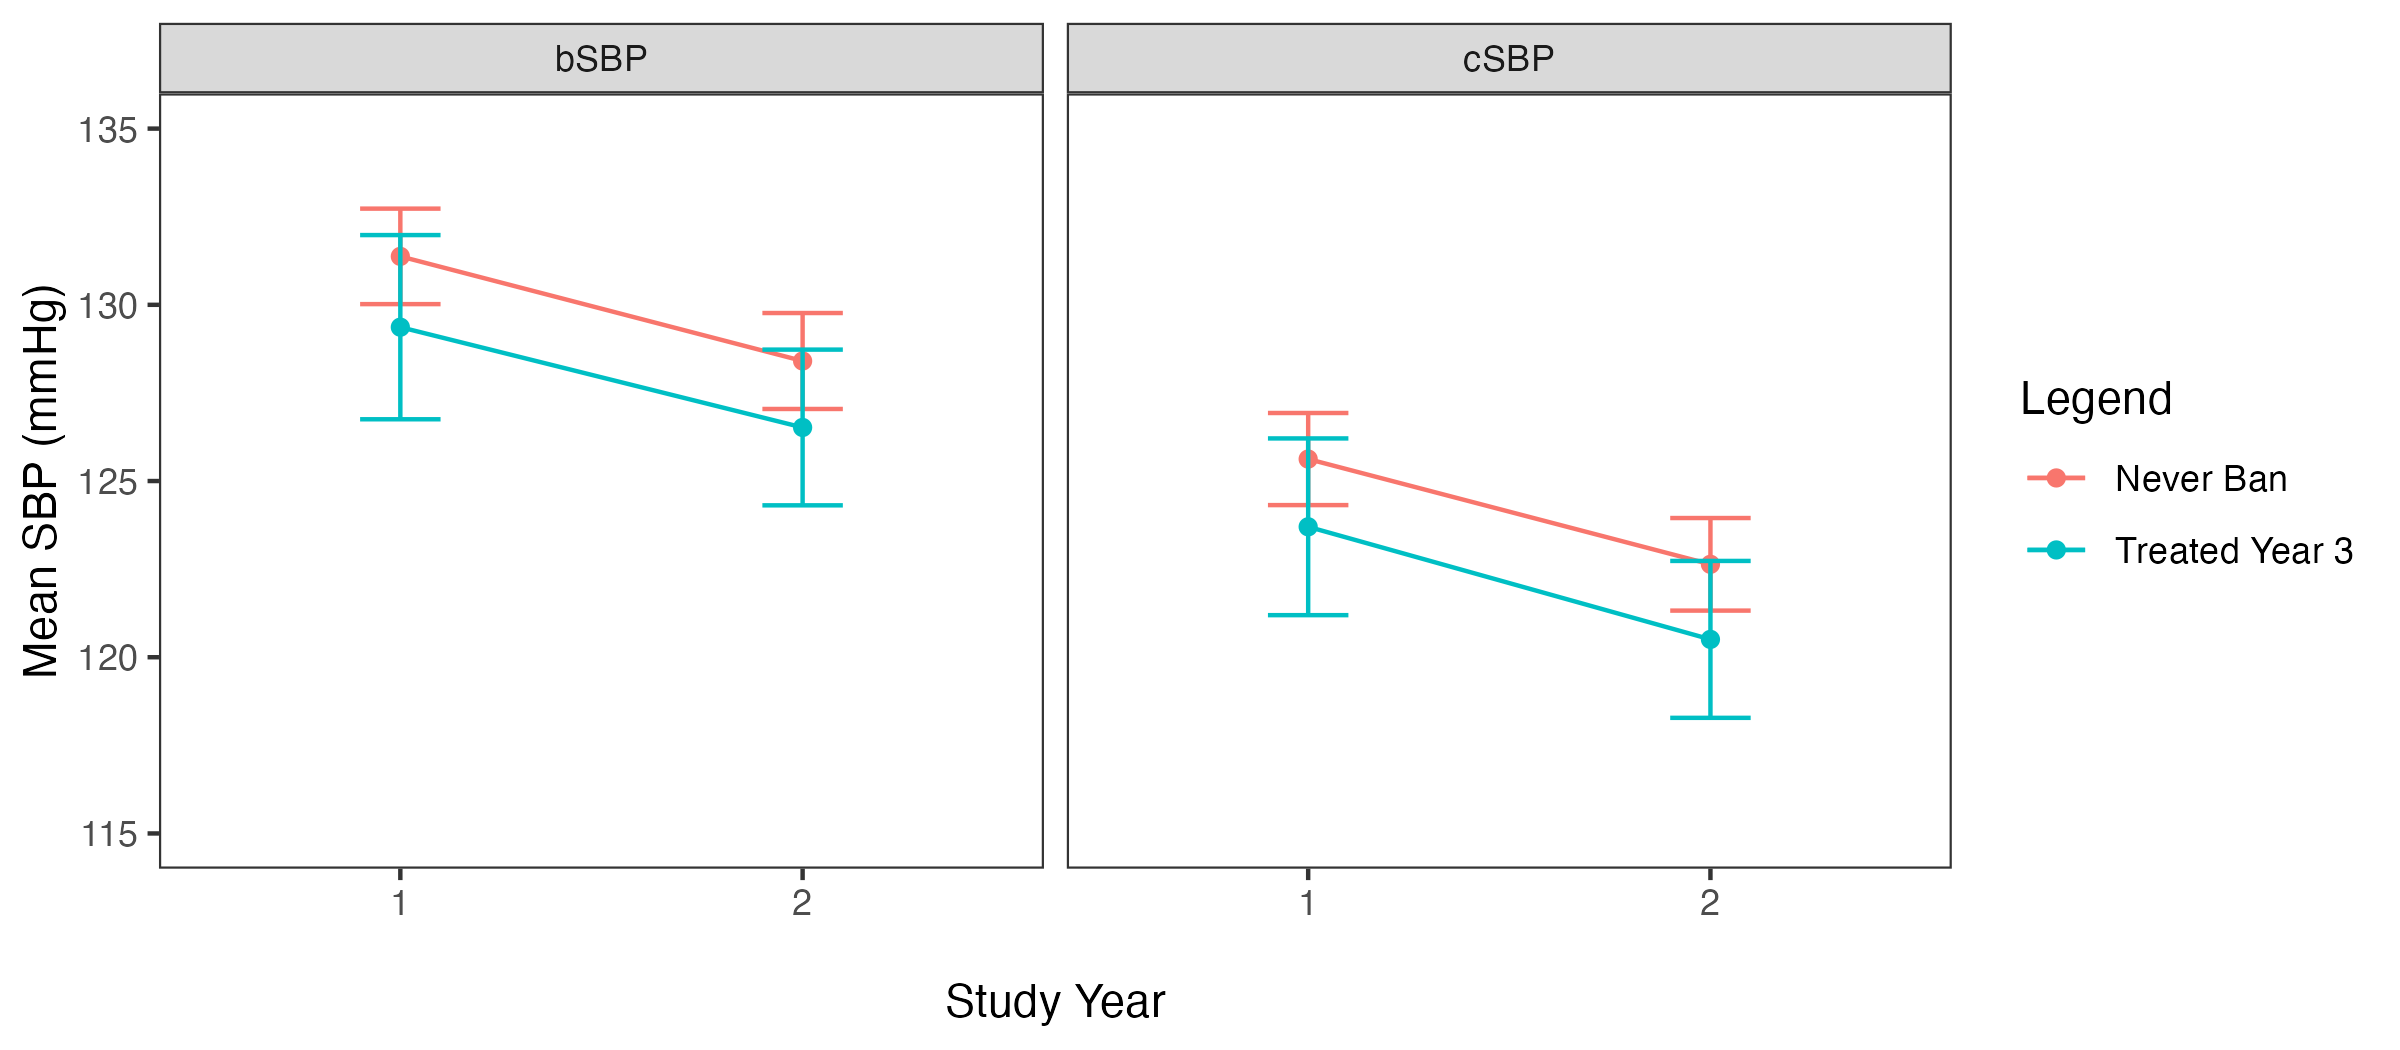
\includegraphics{images/never_Y3_SBP.png}

}

}

\subcaption{\label{fig-afig-pt-1}Treated in W3: Systolic}
\end{minipage}%
\newline
\begin{minipage}[t]{\linewidth}

{\centering 

\raisebox{-\height}{

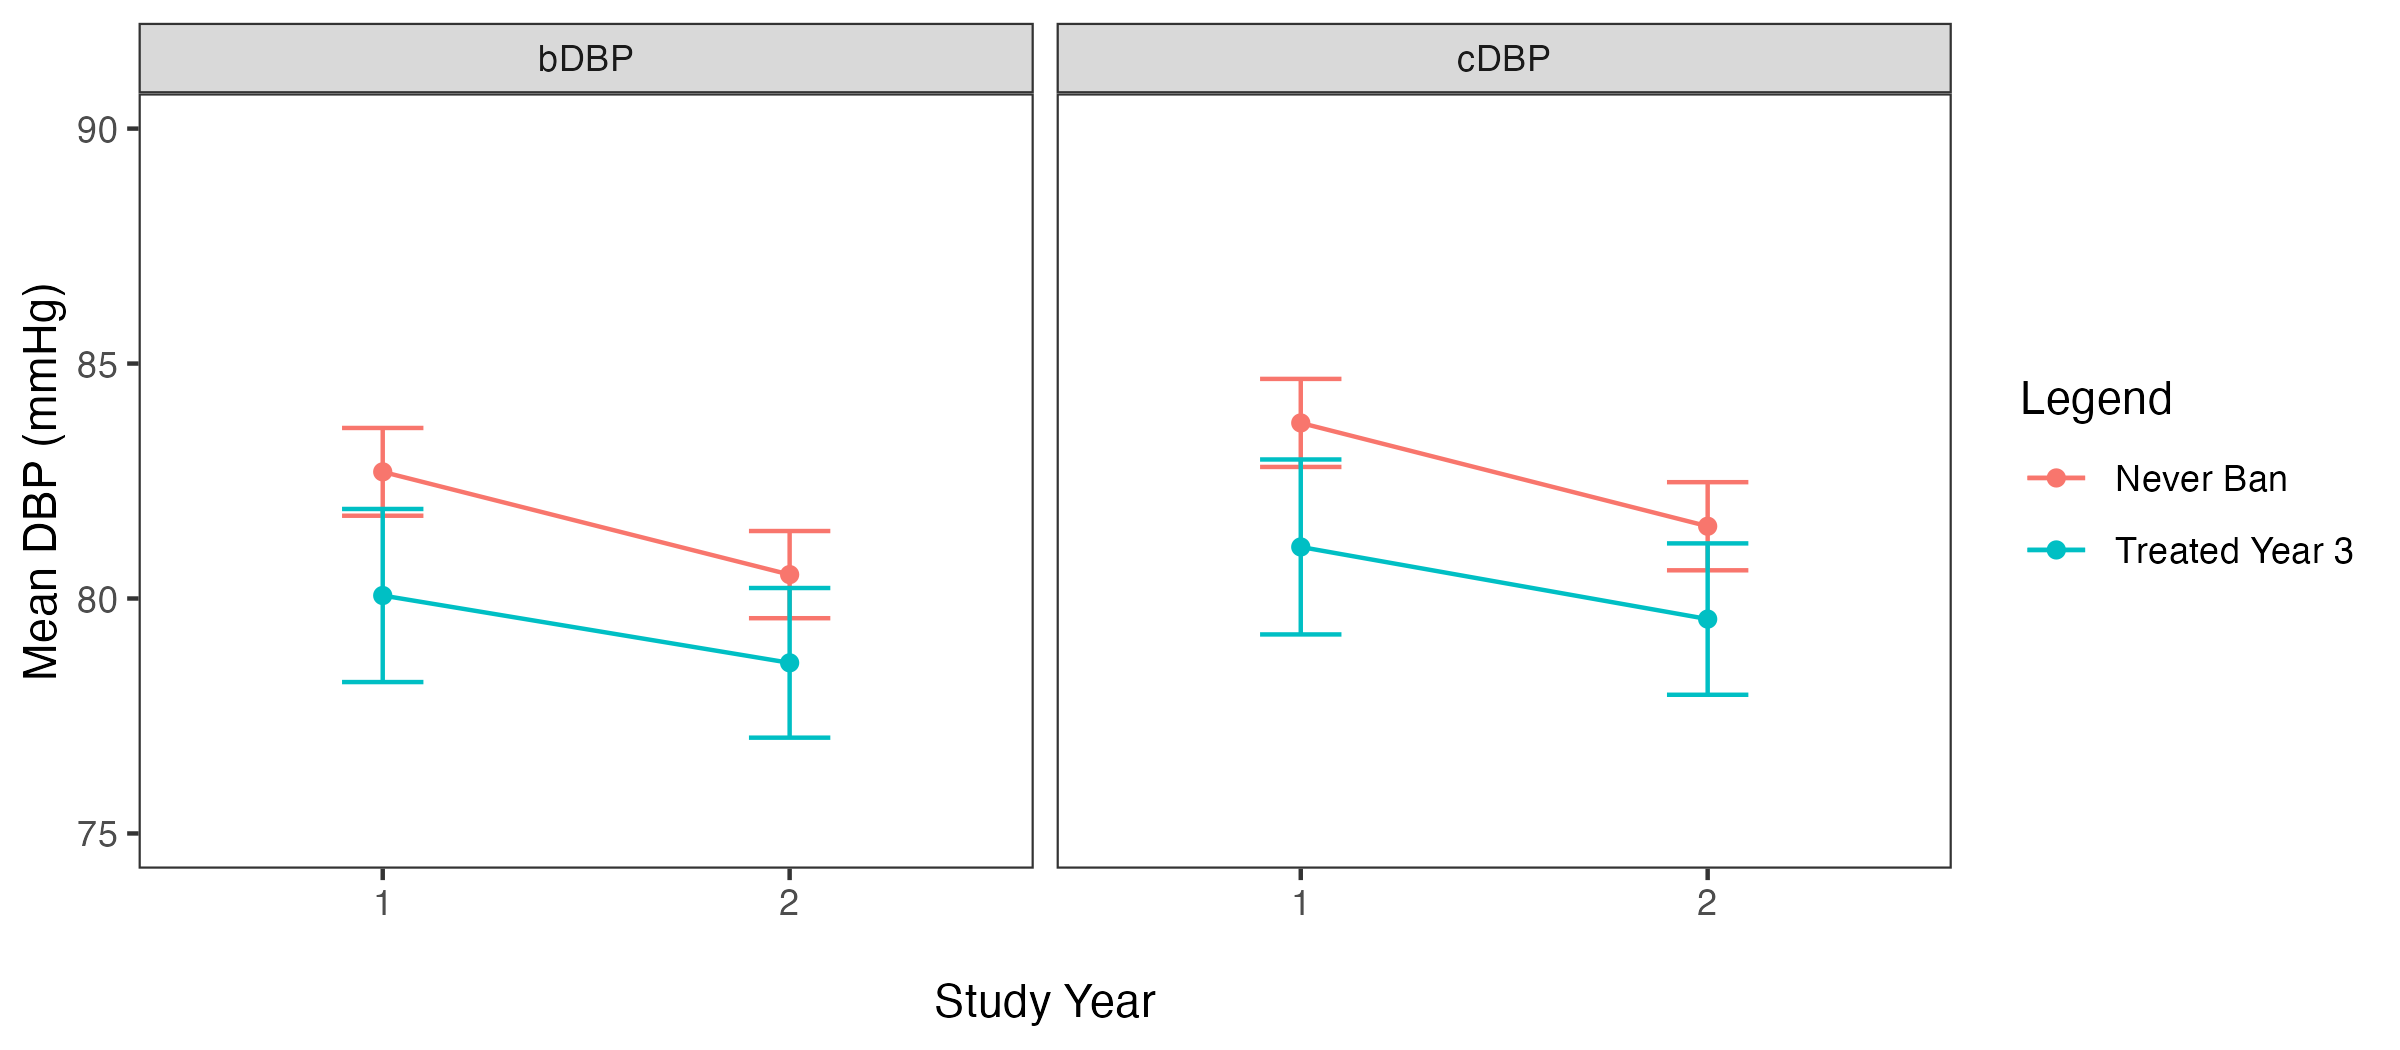
\includegraphics{images/never_Y3_DBP.png}

}

}

\subcaption{\label{fig-afig-pt-2}Treated in W3: Diastolic}
\end{minipage}%
\newline
\begin{minipage}[t]{\linewidth}

{\centering 

\raisebox{-\height}{

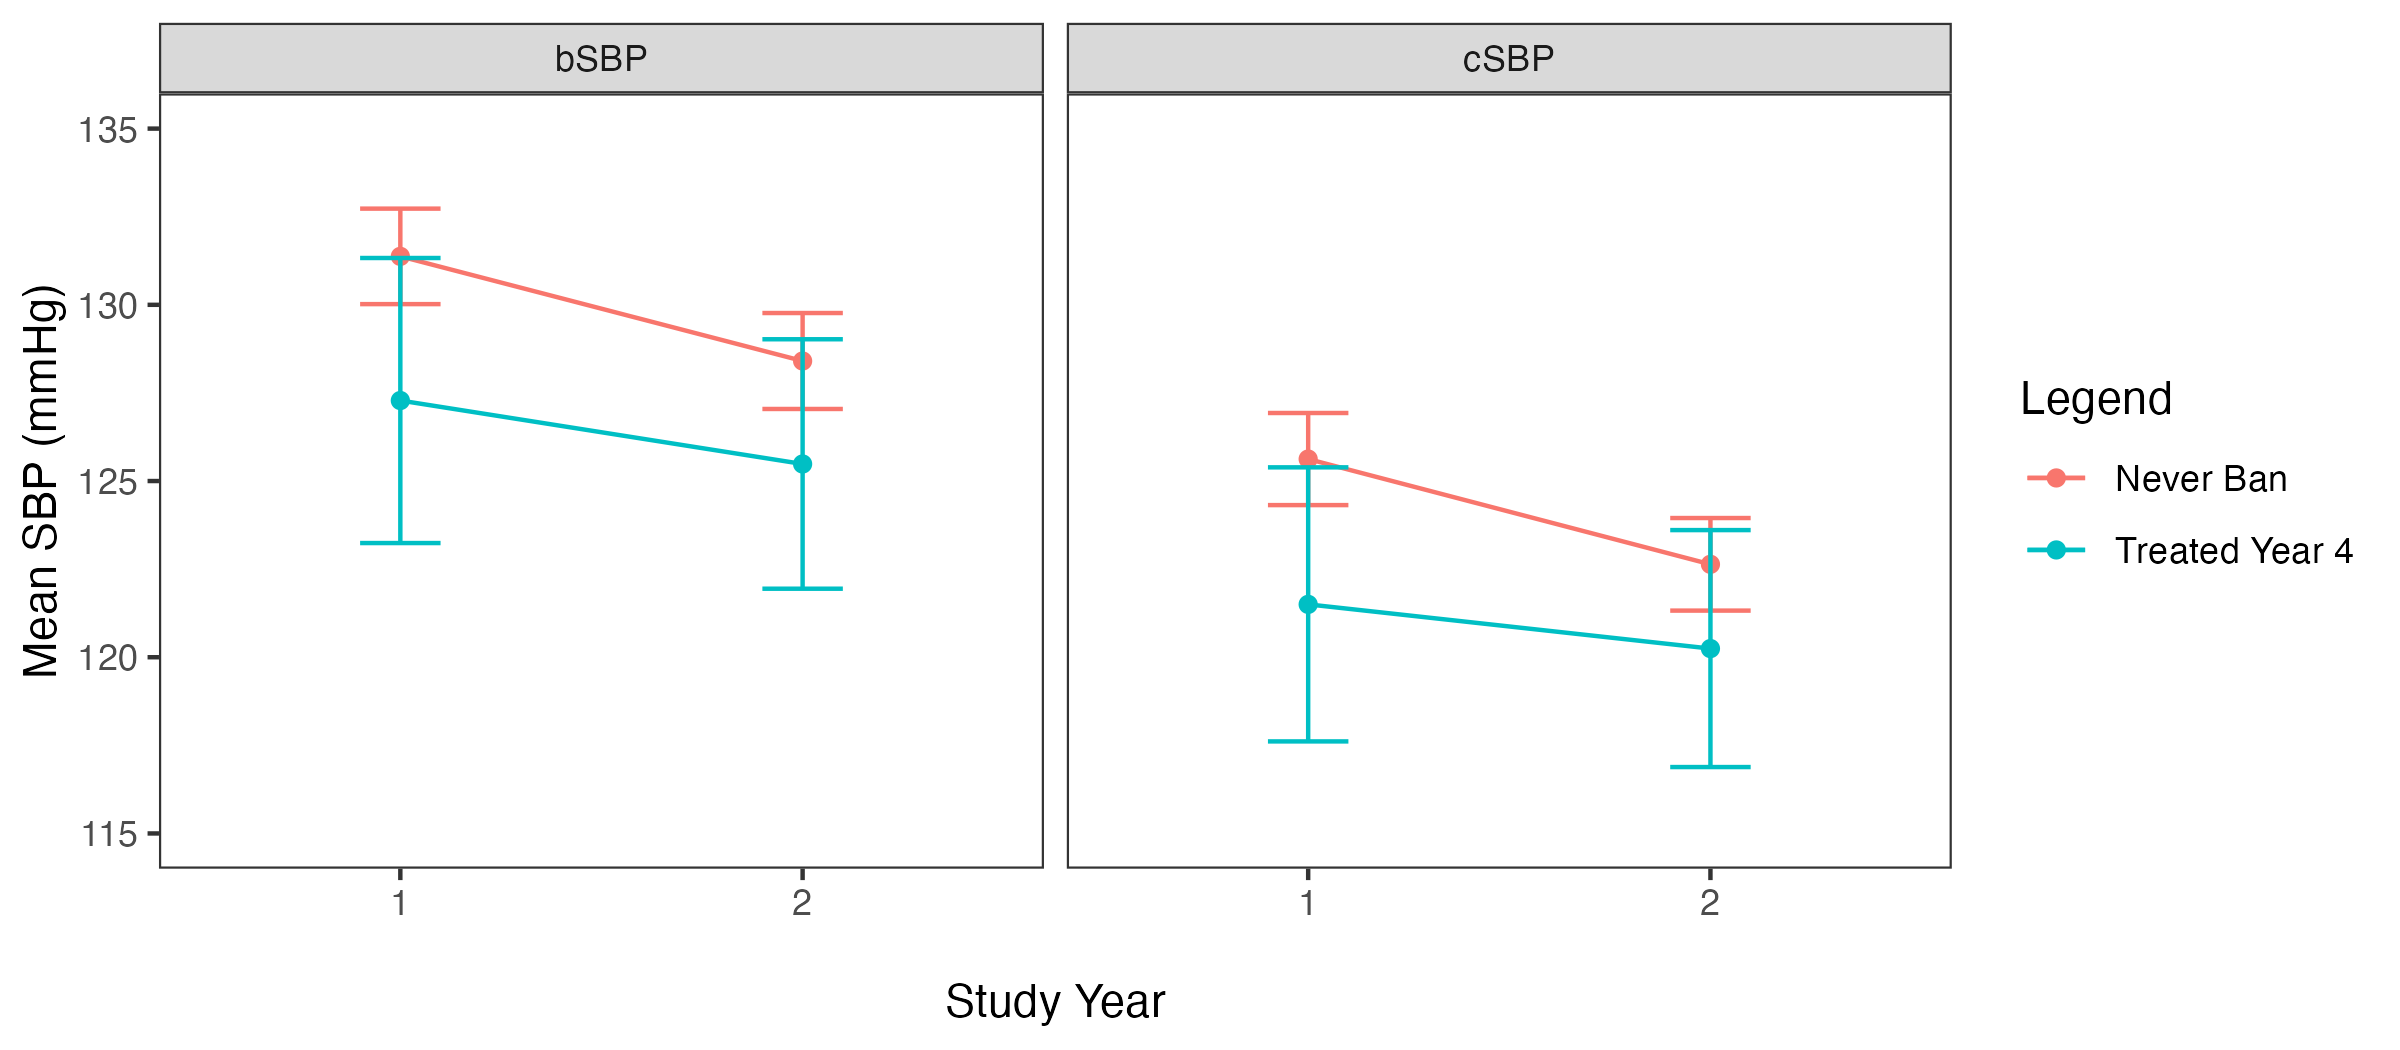
\includegraphics{images/never_Y4_SBP.png}

}

}

\subcaption{\label{fig-afig-pt-3}Treated in W4: Systolic}
\end{minipage}%
\newline
\begin{minipage}[t]{\linewidth}

{\centering 

\raisebox{-\height}{

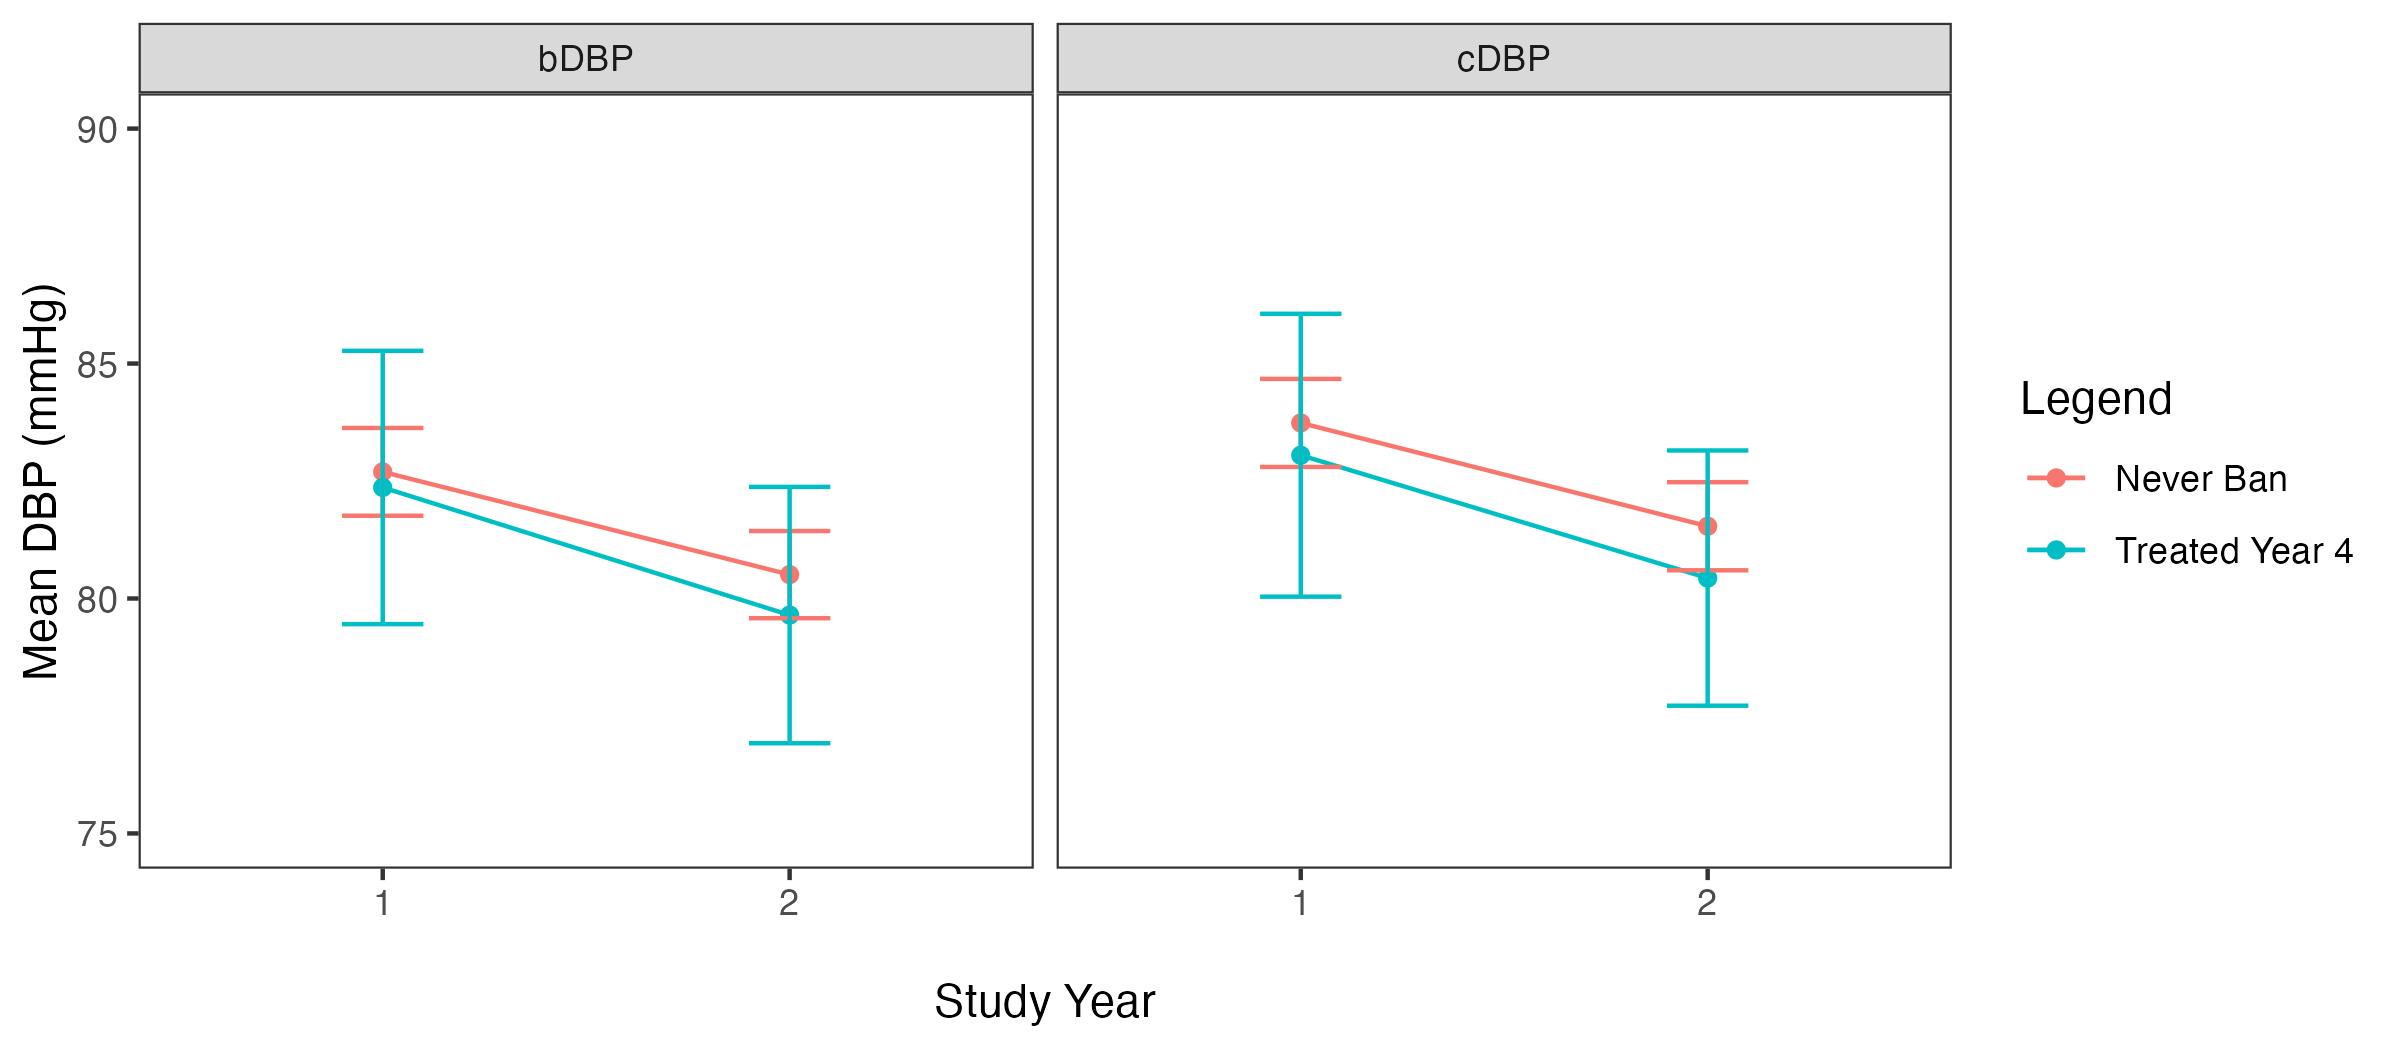
\includegraphics{images/never_Y4_DBP.png}

}

}

\subcaption{\label{fig-afig-pt-4}Treated in W4: Diastolic}
\end{minipage}%

\caption{\label{fig-afig-pt}Comparison of pre-interventions trends in
blood pressure between waves 1 and 2 for never treated and villages
treated in waves 3 and 4.}

\end{figure}



\end{document}
